
\documentclass[10pt]{article}

\usepackage[T1]{fontenc}
\usepackage[utf8]{inputenc}
\usepackage{amssymb}
\usepackage{newtxtext,newtxmath}
\usepackage[letterpaper,left=1.05in,right=1.05in,top=0.72in,bottom=0.78in]{geometry}
\usepackage{booktabs}
\usepackage{array}
\usepackage{tabularx}
\usepackage{graphicx}
\usepackage{amsmath}
\usepackage{enumitem}
\usepackage{xcolor}
\usepackage{xurl}
\usepackage{xspace}
\usepackage{hyperref}
\usepackage{tikz}
\usepackage{caption}
\usepackage{float}
\usepackage{microtype}
\usepackage{titlesec}
\usetikzlibrary{arrows.meta,positioning,fit,calc}

\hypersetup{
  colorlinks=true,
  linkcolor=black,
  citecolor=black,
  urlcolor=blue,
  pdfauthor={Yueyue Zhang},
  pdftitle={EduSkillBench: Measuring the Impact of Agent Skills on Single-Turn Educational Tasks}
}

\setlength{\parindent}{1.35em}
\setlength{\parskip}{0pt}
\setlength{\emergencystretch}{2em}
\renewcommand{\arraystretch}{1.12}
\setlength{\tabcolsep}{5.5pt}
\captionsetup{font=small,labelfont=normalfont,labelsep=colon,skip=4pt}
\setlist[itemize]{leftmargin=1.6em,itemsep=1pt,topsep=3pt}
\setlist[enumerate]{leftmargin=2.0em,itemsep=1pt,topsep=3pt}

\titleformat{\section}{\bfseries\large}{\thesection}{0.55em}{}
\titleformat{\subsection}{\bfseries\normalsize}{\thesubsection}{0.55em}{}
\titleformat{\subsubsection}{\bfseries\normalsize}{\thesubsubsection}{0.5em}{}
\titlespacing*{\section}{0pt}{11pt}{5pt}
\titlespacing*{\subsection}{0pt}{8pt}{3pt}
\titlespacing*{\subsubsection}{0pt}{6pt}{2pt}

\newcommand{\bench}{\textsc{EduSkillBench}\xspace}
\newcommand{\skill}[1]{\texttt{#1}}
\newcommand{\ppgain}[1]{+#1\,pp}
\DeclareRobustCommand{\halfcircle}{\tikz[baseline=-0.5ex,line width=0.09ex]{\draw (0,0) circle (0.5ex);\begin{scope}\clip (0,0) circle (0.5ex);\fill (-0.5ex,-0.55ex) rectangle (0,0.55ex);\end{scope}}}

\begin{document}
\thispagestyle{empty}

\noindent\rule{\textwidth}{3.3pt}
\vspace{0.45em}

\begin{center}
{\bfseries\fontsize{18pt}{20.5pt}\selectfont
EduSkillBench: Measuring the Impact of Agent Skills\\[2pt]
on Single-Turn Educational Tasks}
\vspace{0.55em}

{\normalsize Yueyue Zhang}\\[-1pt]
{\small School of Artificial Intelligence, Anhui University, Hefei, China}\\[-1pt]
{\small Code and data: \url{https://github.com/Airlivy/EduSkillBench}}
\end{center}

\vspace{0.35em}
\noindent\rule{\textwidth}{0.65pt}

\vspace{0.7em}
\begin{center}
{\bfseries Abstract}
\end{center}
\vspace{-0.35em}

Agent Skills are reusable packages of procedural knowledge that augment large language model (LLM) agents at inference time. Educational agents are a natural target for such augmentation, because high-quality teaching behavior depends not only on factual knowledge but also on procedures for diagnosing misconceptions, sequencing hints, designing assessments, differentiating content, and structuring lessons. Existing educational benchmarks mostly measure whether agents can solve educational tasks; they do not isolate how a matched Skill changes the outcome.

We present \bench, a controlled benchmark that evaluates educational Skills under matched No-Skill versus With-Skill conditions. The v1 release curates 18 public education-oriented Skills from two open repositories, maps them to six EduBench-inspired scenarios, and constructs 54 Skill-aligned tasks with explicit task-specific rubrics, of which 42 are single-turn tasks across 14 Skills and 12 are multi-turn tasks across 4 Skills. This paper reports the single-turn subset, evaluated with OpenCode (an agent harness) and BenchFlow (an orchestration framework). On a 0 to 1 rubric-reward scale, the observed mean reward rises from 0.767 to 0.948 for \texttt{qwen3.7-plus} (\ppgain{18.1}) and from 0.314 to 0.557 for \texttt{deepseek-v4-flash} (\ppgain{24.3}). The gains are broad but non-uniform: 10 of 14 Skills improve for Qwen and 9 of 14 for DeepSeek, with one negative-transfer Skill per model, that is, one Skill whose With-Skill reward is lower than its matched No-Skill baseline.

All reported values are single-run point estimates and are presented descriptively. Because each model row is scored by a same-family judge, cross-model comparisons are descriptive rather than causal. \bench~contributes a reproducible benchmark for studying educational Skill efficacy, and its central design limitation, that tasks and rubrics are aligned to the matched Skill, is stated explicitly and made measurable. The multi-turn subset is released as task specifications and is not yet evaluated.

\vspace{0.6em}

\begin{figure}[H]
\centering
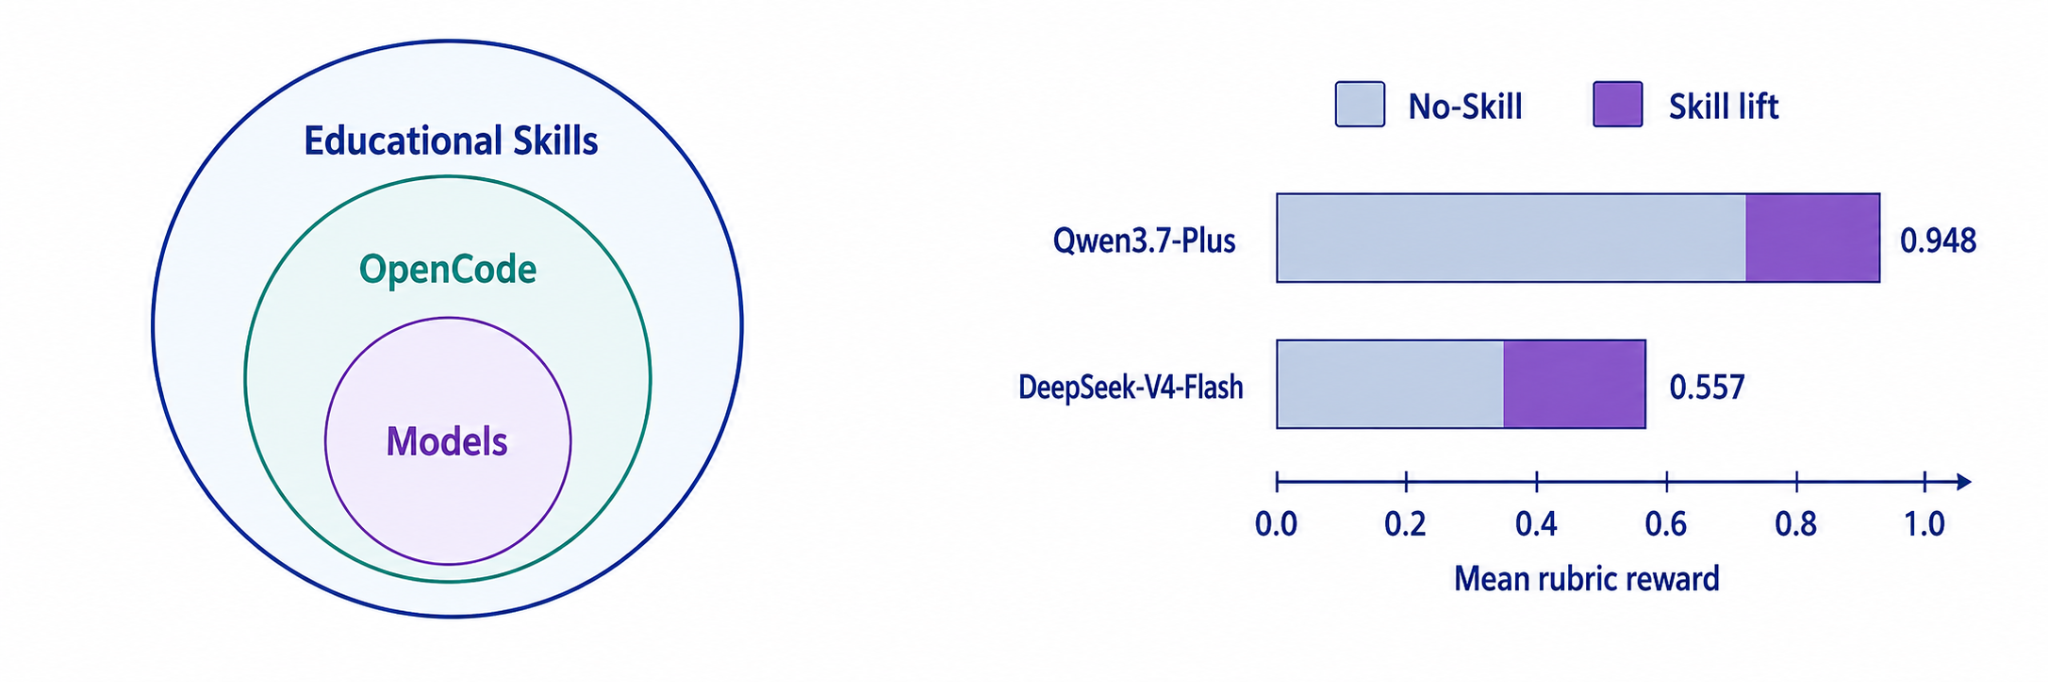
\includegraphics[width=0.94\textwidth]{fig1_overview.png}
\caption{Agent stack and single-turn results in \bench. Each horizontal bar stacks the No-Skill baseline and the observed lift from the matched Skill, where lift is the With-Skill mean rubric reward minus the No-Skill mean rubric reward. Both configurations use the OpenCode harness and the BenchFlow evaluation pipeline.}
\label{fig:overview}
\end{figure}

\newpage

\section{Introduction}

\subsection{Research Questions}

\bench~is designed around three research questions:

\textbf{RQ1, Overall Skill Effectiveness.}
Do educational Agent Skills improve LLM agent performance compared with the same agent without Skill access?

\textbf{RQ2, Cross-model Generalization.}
Are Skill-induced improvements consistent across different LLM backbones?

\textbf{RQ3, Skill-level Transferability.}
Which educational Skills provide reliable positive transfer, and when can Skills introduce limited or negative transfer, where negative transfer means a Skill that lowers observed reward relative to its matched No-Skill baseline?


LLM agents are increasingly used for education-facing work, including lesson planning, formative assessment, tutoring, differentiation, project design, retrieval practice, and learning-support workflows. A fundamental tension follows. Foundation models contain broad educational knowledge, but many high-quality teaching behaviors are procedural: a tutor must decide when to withhold an answer, how to escalate a hint, how to diagnose a misconception, or how to translate a learning objective into an aligned assessment. These procedures are difficult to capture with factual retrieval alone.

Agent Skills provide an inference-time mechanism for supplying reusable procedures. A Skill typically contains a \texttt{SKILL.md} file with instructions and may include templates, references, scripts, or worked examples. Unlike fine-tuning, Skill augmentation does not modify model weights. Unlike ordinary prompting, Skills are intended to be modular and reusable across task instances. \bench~operationalizes Skill access as adding the matched Skill package to the agent context, so its experiment measures the effect of adding a matched Skill relative to no added instructions. It does not, by itself, separate the Skill as a reusable package from the general effect of adding task-relevant instruction text; that separation is a required validation step (Section~6.1).

The benchmark problem is therefore different from ordinary education evaluation. EduBench asks whether a model performs well across diverse educational scenarios and introduces multidimensional educational criteria \cite{edubench}. SkillsBench asks whether curated Agent Skills improve agents on matched tasks and establishes paired No-Skill versus With-Skill evaluation as a central design \cite{skillsbench}. \bench~lies at the intersection: it asks how to construct and score education-specific tasks when the evaluated system is an LLM agent augmented with reusable Skills.

We make four contributions:
\begin{enumerate}
  \item \textbf{Education-specific Skill benchmark.} We curate 18 public educational Skills from two open repositories and map them to six of the nine EduBench-inspired scenarios. The curation is a data and engineering contribution, not a new evaluation method.
  \item \textbf{Skill-aligned tasks and rubrics.} We construct 54 benchmark tasks, each with explicit context, user request, expected output, and rubric, and we state explicitly that the tasks and rubrics are written around the behavior each Skill claims to support. The alignment is deliberate and disclosed, and its effect on the measured lift is a first-class quantity of the benchmark rather than a hidden confound.
  \item \textbf{Reproducible cross-model single-turn evidence.} We report 168 clean single-turn runs across two model configurations. Skills are associated with an average reward increase of \ppgain{18.1} for \texttt{qwen3.7-plus} and \ppgain{24.3} for \texttt{deepseek-v4-flash}, while per-Skill effects remain highly heterogeneous. All values are single-run point estimates reported descriptively.
  \item \textbf{An explicit validation agenda.} We specify the experiments required to move from descriptive observation to causal and uncertainty-bounded claims, including repeated runs, a common judge, and instruction-level controls (Section~6.1).
\end{enumerate}

We adopt, rather than introduce, the paired No-Skill versus With-Skill design established by SkillsBench \cite{skillsbench}. The goal of \bench~is not to claim that every Skill is beneficial. Rather, it provides a structured way to ask whether a Skill helps, where it helps, and when it can hurt.

\section{Background}

\textbf{Skill definition.}
Following the emerging Agent Skills convention, we define a Skill as a reusable, file-based package of procedural guidance for a class of tasks. A Skill can specify sequencing rules, constraints, heuristics, templates, references, or execution aids. It is distinct from model weights and becomes actionable only through a compatible agent harness.

\textbf{Skill augmentation.}
We use Skill augmentation to denote the inference-time condition in which a matched Skill is made available to the agent. For \bench, the experimental contrast is deliberately narrow: the same task is run with and without that Skill, and the matched Skill is present only in the With-Skill arm.

\textbf{Educational evaluation.}
Open-ended educational outputs are rarely reducible to exact-match scoring. A lesson plan can be factually correct but poorly aligned with its objective; a hint can be correct but pedagogically premature. We therefore use task-specific rubrics with explicit expected behaviors, following the broader practice of rubric-based LLM evaluation \cite{llmjudge}.

Table~\ref{tab:augmentation} situates Skill augmentation among runtime augmentation paradigms. A check mark ($\checkmark$) means the paradigm fully provides the capability, a partial mark (\halfcircle) means it provides it partially or indirectly, and a cross ($\times$) means it does not provide it. The column ordering runs from Prompting, to RAG, to Tools, to Skills. Skills are the only paradigm that simultaneously packages reusable procedural guidance and remains portable across model configurations, which is the property \bench~is designed to measure.

\begin{table}[H]
\centering
\small
\caption{Runtime augmentation paradigms relevant to educational agents. $\checkmark$ = fully supports, \halfcircle = partially supports, $\times$ = does not support.}
\label{tab:augmentation}
\begin{tabular}{lcccc}
\toprule
 & Prompting & RAG & Tools & Skills \\
\midrule
Reusable package & $\times$ & \halfcircle & $\times$ & $\checkmark$ \\
Procedural guidance & \halfcircle & $\times$ & \halfcircle & $\checkmark$ \\
External factual context & $\times$ & $\checkmark$ & varies & varies \\
Executable resources & $\times$ & $\times$ & $\checkmark$ & optional \\
Cross-model portability & $\checkmark$ & $\checkmark$ & $\times$ & $\checkmark$ \\
\bottomrule
\end{tabular}
\end{table}

\section{\bench}

A benchmark for Skill-augmented education is only useful if the Skills, tasks, and rubrics are separable enough to avoid reducing evaluation to prompt imitation. \bench~therefore treats benchmark construction as part of the contribution.

\subsection{Design Principles}

\textbf{Public Skills, not benchmark-authored interventions.}
All 18 retained Skills originate from existing public repositories. Missing scenario coverage is left missing rather than filled with newly authored benchmark-specific Skills.

\textbf{Scenario-grounded tasks.}
Tasks instantiate recognizable teacher- or learner-facing educational work, using the EduBench scenario taxonomy as an organizing scaffold.

\textbf{Observable procedures.}
A retained Skill must encode behavior that can be observed in an output or interaction and judged through explicit criteria.

\textbf{Paired conditions.}
No-Skill and With-Skill runs use the same task and model configuration. The only intended experimental difference is access to the matched Skill.

\subsection{Construction Pipeline}

\begin{figure}[H]
\centering
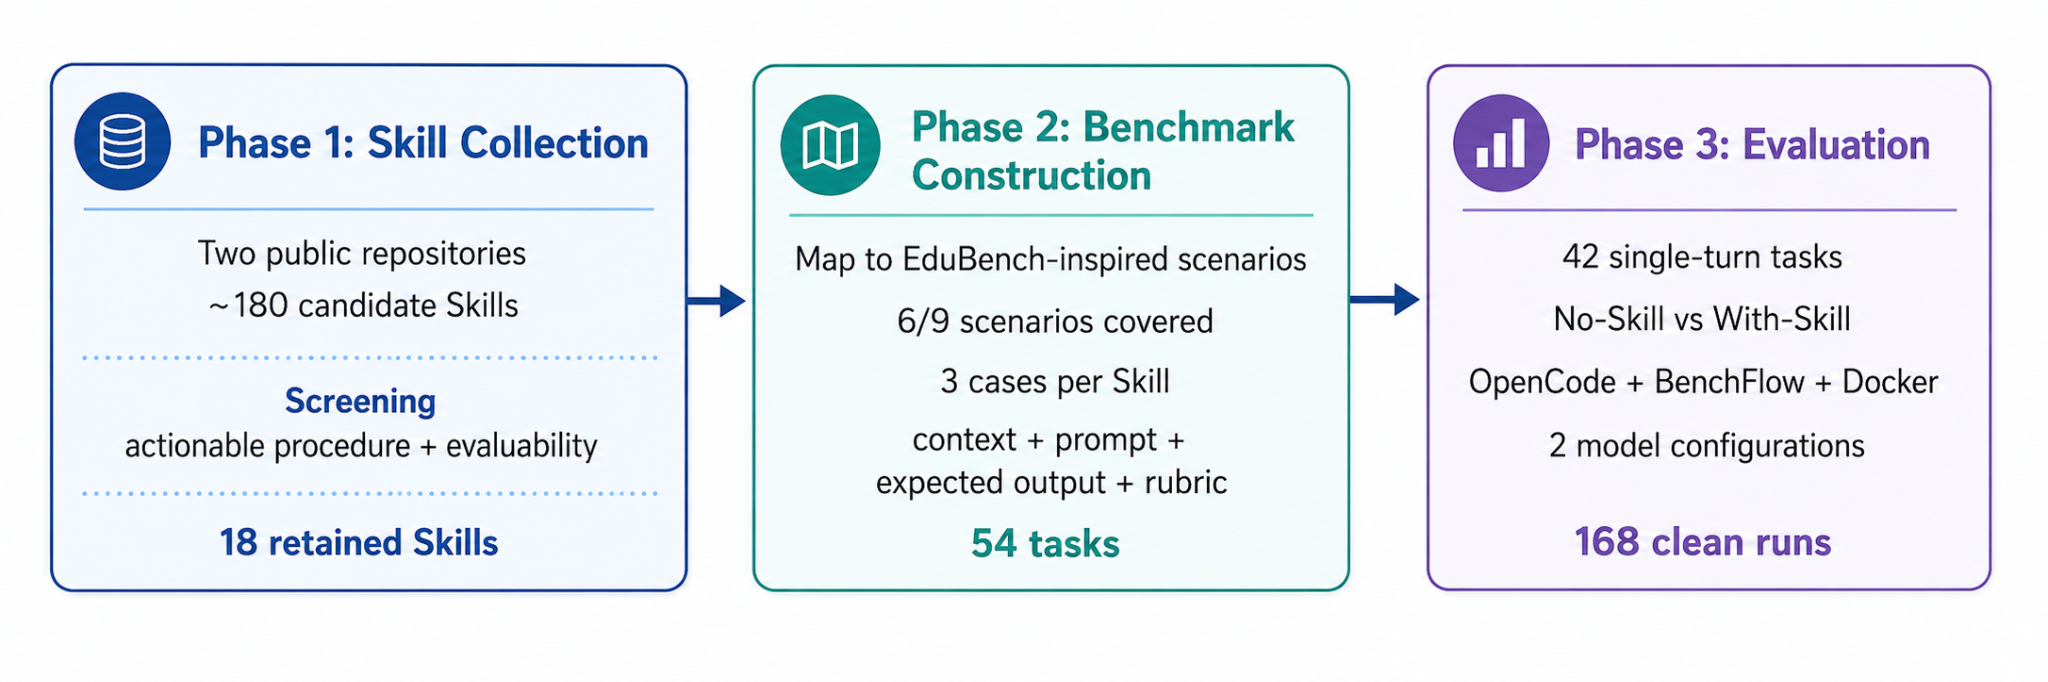
\includegraphics[width=0.94\textwidth]{fig2_pipeline.png}
\caption{\bench~pipeline. The benchmark starts from public educational Skills, constructs Skill-aligned tasks and rubrics, and evaluates matched conditions under a fixed agent harness.}
\label{fig:pipeline}
\end{figure}

\subsection{Skill Sources and Filtering}

We source candidate Skills from the Education Agent Skills Library and the Teaching Skills repository \cite{educationagentskills,teachingskills}. At collection time they contain approximately 165 and 15 Skills, respectively. We retain a Skill when it (i) encodes a recognizable educational procedure, (ii) can be instantiated as a self-contained task, (iii) admits explicit rubric-based evaluation, and (iv) maps meaningfully to an education scenario.

The final pool contains 18 Skills: 14 single-turn and 4 multi-turn. They cover six EduBench-inspired scenarios. We retain no suitable public Skill for Idea Provision, Emotional Support, or Automatic Grading; these gaps are preserved rather than filled artificially.

\subsection{Task Specification}

Each retained Skill is paired with three cases, intentionally varying subject, educational level, and difficulty. The released task schema includes:
\begin{center}
\texttt{task\_id, skill\_id, scenario, subject, education\_level, difficulty, context, user\_prompt, expected\_output, rubric}.
\end{center}

For the 14 single-turn Skills, each Skill contributes one easy, one medium, and one hard case, yielding 14 tasks at each difficulty level. The multi-turn subset targets interaction-dependent procedures such as retrieval-first gating, error diagnosis, progressive hinting, and confidence calibration. Its 12 task specifications are released, but a dedicated stateful evaluation protocol is not yet implemented, so the reported experiment covers the single-turn subset only.

\begin{table}[H]
\centering
\caption{Summary of \bench~v1.}
\label{tab:summary}
\begin{tabular}{lr}
\toprule
Statistic & Count \\
\midrule
Public Skill source repositories & 2 \\
Candidate Skills & 180 \\
Selected Skills & 18 \\
Single-turn Skills & 14 \\
Multi-turn Skills & 4 \\
Single-turn tasks & 42 \\
Multi-turn tasks & 12 \\
Total tasks & 54 \\
EduBench-inspired scenarios covered & 6 / 9 \\
Single-turn tasks evaluated & 42 \\
\bottomrule
\end{tabular}
\end{table}

\subsection{Rubric System}

The central evaluation artifact in \bench~is not only the prompt, but the \emph{task-specific rubric}. Single-turn cases operationalize the target educational procedure as five explicit expected behaviors. Typical criteria include task fulfillment, pedagogical appropriateness, adherence to the intended procedure, actionability, diagnostic quality, alignment with learning objectives, or accessibility constraints. The final reward is normalized to the $[0,1]$ interval.

The rubrics are intentionally sample-specific rather than a single universal checklist. A hinge-question task must reward diagnostic distractors and actionable teaching decisions, while a lesson-building task must reward objective alignment, timings, materials, facilitation, and contingency planning. Multi-turn rubrics additionally require state tracking and response adaptation.

Conceptually, these criteria fall into four evaluation families:
\begin{itemize}
  \item \textbf{Task fulfillment:} whether the requested artifact or response is complete and correct;
  \item \textbf{Pedagogical quality:} whether the output is instructionally appropriate for the learner and objective;
  \item \textbf{Skill execution quality:} whether the procedure targeted by the matched Skill is actually expressed in the output;
  \item \textbf{Interaction quality:} for multi-turn tasks, whether the agent adapts across learner responses rather than applying a static script.
\end{itemize}
The current single-turn experiment scores the first three through the released expected-behavior rubrics; multi-turn interaction quality is released as task specification but not yet included in the reported experiment.

Because the single-turn reward includes the Skill execution family, the measured lift is a \emph{Skill-aligned utility}: it can reward output that expresses the matched procedure even when independent pedagogical quality is unchanged. This is the intended scope of v1, and it means the headline lift can overstate a Skill's contribution relative to a procedure-free rubric. Quantifying the contribution of the Skill execution family, and validating the rubrics against independent human judgment, are required validation steps (Section~6.1).

\subsection{Anatomy of an \bench~Task}

\begin{figure}[H]
\centering
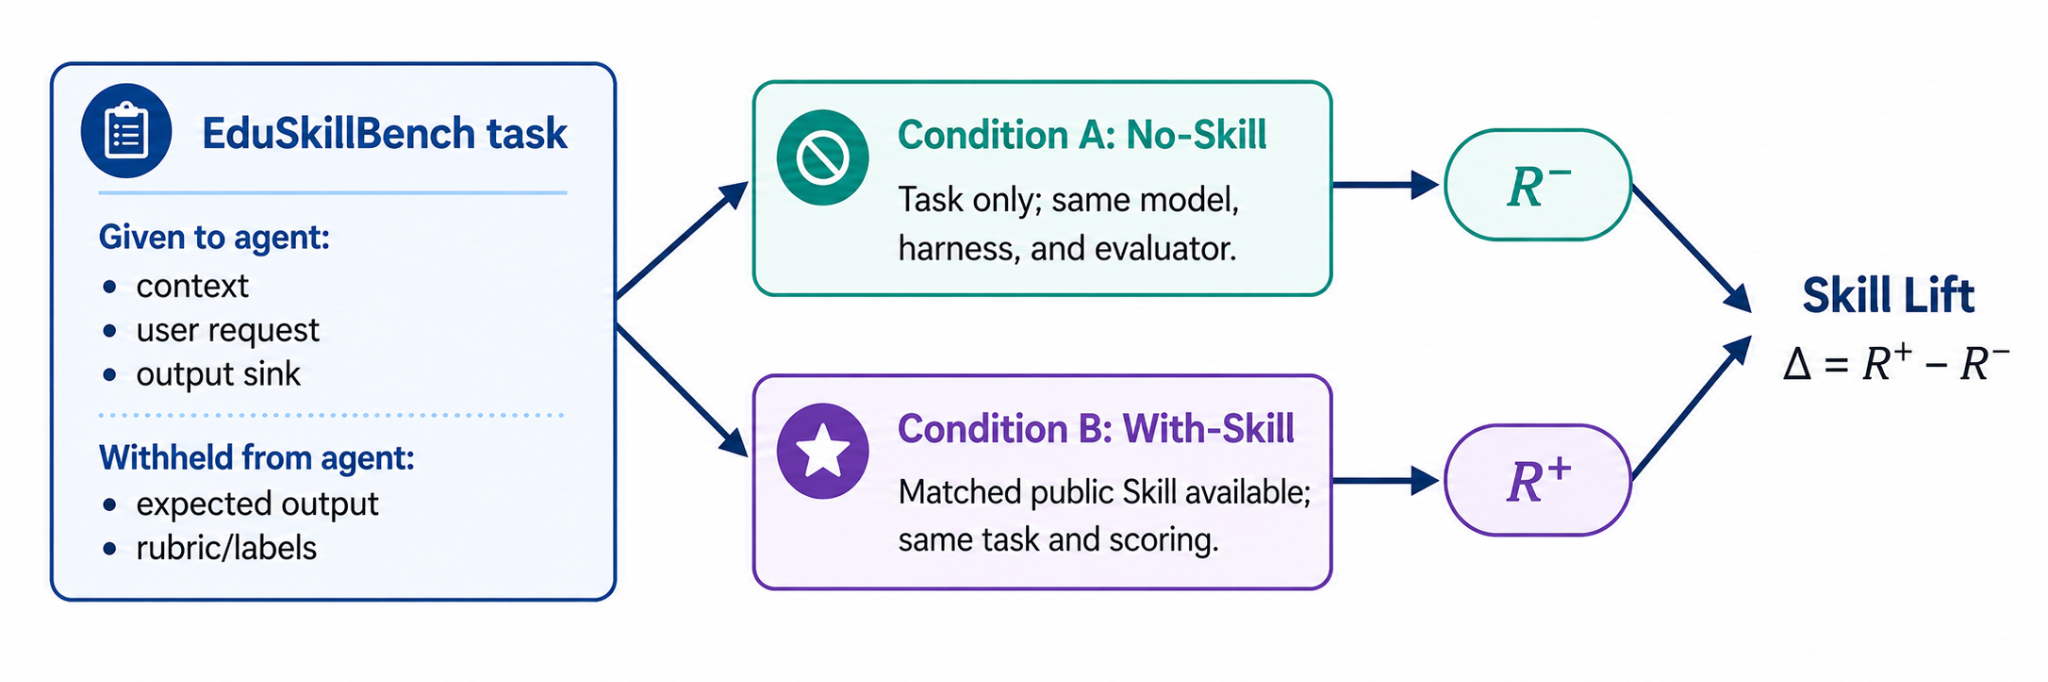
\includegraphics[width=0.94\textwidth]{fig3_anatomy.png}
\caption{Anatomy of a \bench~single-turn evaluation. The task and scoring rubric are fixed; the two arms differ only in access to the matched Skill.}
\label{fig:anatomy}
\end{figure}

\subsection{Educational Skill Taxonomy}

To analyze the coverage of educational procedures, we categorize collected Skills into six functional groups: instruction design (e.g., lesson planning), learning strategy (e.g., retrieval practice), assessment support (e.g., hinge questions), student support (e.g., self-efficacy and motivation), questioning and reasoning (e.g., Socratic questioning), and project learning (e.g., project scaffolding).

This taxonomy is not intended as a new educational ontology. Instead, it provides a structured view of the procedural knowledge represented in \bench~and enables analysis of whether Skill effects differ across educational functions.

\subsection{Benchmark Composition}

The six covered EduBench-inspired scenarios are distributed unevenly because coverage follows the available public Skill ecosystem rather than a quota. The six scenarios are Question Generation (writing questions and diagnostic items), Personalized Content Creation (adapting content to a learner), Teaching Material Generation (building lessons, plans, and teaching resources), Q\&A (answer-first gated dialogue), Error Correction (diagnosing and correcting learner mistakes), and Personalized Learning Support (adaptive and calibrated tutoring sequences). The evaluated single-turn subset covers the first three: Question Generation, Personalized Content Creation, and Teaching Material Generation. The released multi-turn subset adds Q\&A, Error Correction, and Personalized Learning Support.

\begin{figure}[H]
\centering
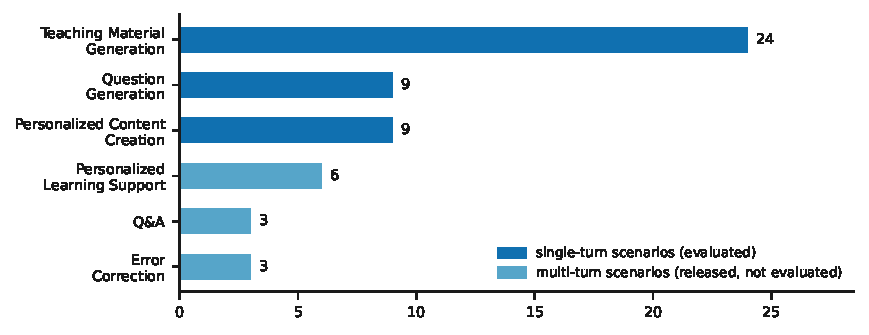
\includegraphics[width=0.92\textwidth]{figure_4.pdf}
\caption{Task composition across the six covered EduBench-inspired scenarios. Counts include both single-turn and multi-turn task specifications. Teaching Material Generation contributes 24 tasks, Question Generation 9, Personalized Content Creation 9, Personalized Learning Support 6, Q\&A~3, and Error Correction 3, for 54 total.}
\label{fig:composition}
\end{figure}

\section{Experiment}

\subsection{Models, Harness, and Conditions}

We evaluate two model configurations: \texttt{qwen3.7-plus} (Qwen, a general-purpose LLM family) and \texttt{deepseek-v4-\allowbreak flash} (DeepSeek, another general-purpose LLM family). Both use OpenCode, an open agent harness, as the agent runtime; BenchFlow, an orchestration framework, to create task environments and Docker sandboxes for execution; and Docker for sandboxing. Each of the 42 single-turn tasks is evaluated under two matched conditions: No-Skill and With-Skill. This produces $42\times2=84\allowbreak$ runs per model and 168 clean runs in the final aggregate.

The judge model follows the model configuration used for each run: Qwen results use the Qwen judge identifier, while DeepSeek results use the DeepSeek judge identifier. This design makes each model's paired lift internally interpretable, but it also means the model variable and the judge variable are confounded across rows. We therefore treat cross-model comparisons as descriptive and do not claim a causal reading of cross-model differences; a shared independent judge is a required validation step (Section~6.1).

The No-Skill arm adds no matched instruction text. The design therefore measures the effect of making a matched Skill available relative to no added instructions. It does not separate the Skill as a reusable package from the effect of adding task-relevant instruction text of comparable length. A matched-length, non-matched instruction control is a required validation step (Section~6.1).

\subsection{Evaluation Protocol}

BenchFlow creates the task environment, passes the prompt to the OpenCode agent, and makes the matched Skill available only in the With-Skill arm. The evaluator scores the final response against the case-specific expected behaviors. For DeepSeek, four initial With-Skill runs hit a 300-second wall-clock timeout; those four cells were rerun with a 600-second timeout, and the successful replacements are used in the final 84/84 clean aggregate. Because only the With-Skill cells received the extension, those four lifts could be biased in the With-Skill direction; a sensitivity check under a uniform timeout is a required validation step (Section~6.1).

\subsection{Metrics}

Our primary metric is mean normalized rubric reward. For task $x$, model $M$, agent harness $A$, and matched Skill $s$, the No-Skill reward is
\begin{equation}
R^{-}(x) = R\bigl(A(M, x)\bigr),
\label{eq:reward}
\end{equation}
where $R$ is the rubric reward normalized to $[0, 1]$, and $A(M, x)$ denotes the final output produced by running harness $A$ with model $M$ on task $x$. The With-Skill reward, in which the matched Skill $s$ is also made available to the agent, is
\begin{equation}
R^{+}(x, s) = R\bigl(A(M, x, s)\bigr).
\label{eq:rewardwith}
\end{equation}
The task-level Skill lift is
\begin{equation}
\Delta(x, s) = R^{+}(x, s) - R^{-}(x).
\label{eq:lift}
\end{equation}
For each Skill, we average $\Delta$ over its three cases. Because each evaluated Skill contributes exactly three tasks, macro-averaging over Skills and equal-weight averaging over tasks are equivalent up to rounding.

To mirror the headroom-aware analysis used in SkillsBench \cite{skillsbench}, we also report normalized gain \cite{hake}:
\begin{equation}
g = \frac{\bar{R}^{+} - \bar{R}^{-}}{1 - \bar{R}^{-}},
\label{eq:gain}
\end{equation}
where $\bar{R}^{+}$ and $\bar{R}^{-}$ are the Skill-level macro-averaged With-Skill and No-Skill rewards, and $g$ measures the fraction of remaining score headroom closed by Skill augmentation. We treat $g$ as descriptive, because each model uses its own judge configuration.

All reported values are single-run point estimates. Following the v1 release scope, we report them descriptively and do not attach confidence intervals or significance tests to them. Bounding these estimates with repeated runs is a required validation step (Section~6.1).

\section{Results}

We first report overall efficacy across the two model configurations, then analyze scenario-level and Skill-level heterogeneity. Every number below is a single-run point estimate; we use the word ``observed'' where an interpretation would otherwise sound causal.

\subsection{Overall Skill Effectiveness and Cross-model Transfer}

\subsubsection{Main Results}

\begin{table}[H]
\centering
\caption{Mean normalized rubric reward (0 to 1 scale), absolute Skill lift in percentage points (pp), normalized gain $g$ in percent, and per-Skill outcome counts on the 42-task single-turn subset. Each model has 84 clean runs: 42 No-Skill and 42 With-Skill. All values are single-run point estimates.}
\label{tab:mainresults}
\begin{tabular}{lccccc}
\toprule
Model & No-Skill & With-Skill & $\Delta$ (pp) & $g$ (\%) & Pos./Tie/Neg. Skills \\
\midrule
Qwen3.7-Plus & 0.767 & \textbf{0.948} & +18.1 & 77.7 & 10 / 3 / 1 \\
DeepSeek-V4-Flash & 0.314 & \textbf{0.557} & +24.3 & 35.4 & 9 / 4 / 1 \\
\bottomrule
\end{tabular}
\end{table}

\textbf{Finding 1 (observed): Skills provide broad but non-uniform gains.}
Both model configurations improve substantially in observed mean reward, but the gains differ in magnitude and distribution. Qwen reaches the stronger absolute With-Skill score (0.948), while DeepSeek shows the larger absolute lift (+0.243). Thus, high final performance and high marginal benefit from Skills are not the same property.

\textbf{Finding 2 (observed): Skill benefit depends on the model.}
The same Skill can behave very differently across models. \skill{lesson-builder} rises from 0.200 to 0.933 for Qwen ($+0.733$) but falls from 0.267 to 0.000 for DeepSeek ($-0.267$). Conversely, \skill{retrieval-practice-generator} improves by $+0.267$ for Qwen and by $+0.867$ for DeepSeek. These observed reversals are consistent with treating Skill quality as model-dependent, but they rest on single-run cells scored by model-specific judges, so they are descriptive until the common-judge and repeated-run validations in Section~6.1 are complete.

\textbf{Finding 3 (observed): Ceiling effects can hide useful Skills.}
Three Qwen Skills tie at 1.000 in both conditions. When the baseline already saturates the rubric, the benchmark cannot measure additional benefit even if the Skill improves reasoning or consistency. This motivates harder cases and trajectory-level diagnostics in future releases.

\begin{figure}[H]
\centering
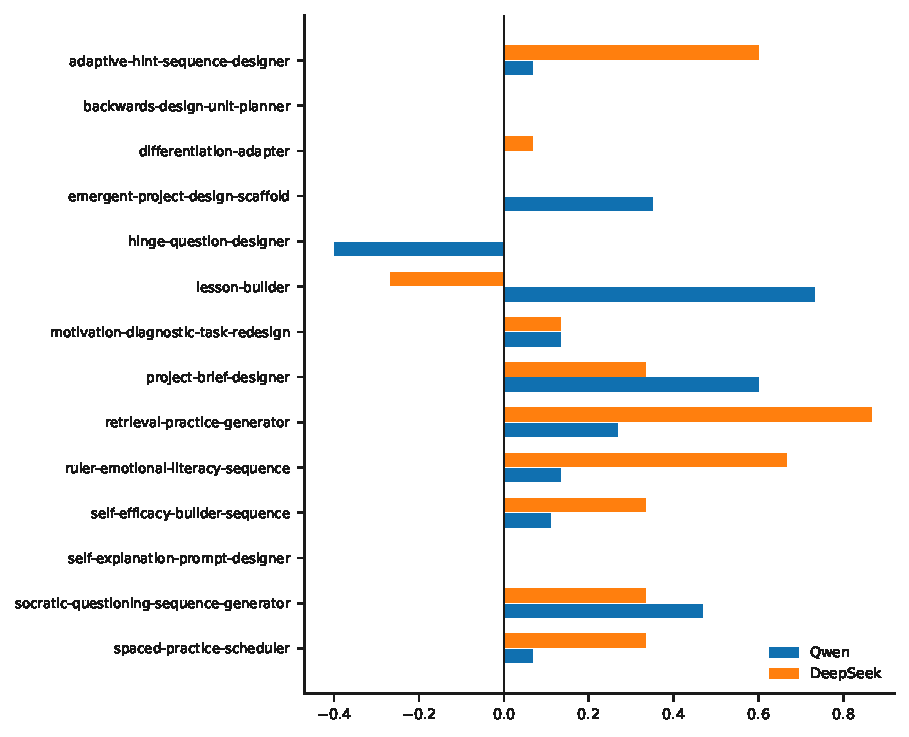
\includegraphics[width=0.94\textwidth]{figure_5.pdf}
\caption{Per-Skill lift for Qwen3.7-Plus and DeepSeek-V4-Flash. Positive values favor the matched Skill condition; negative values indicate observed negative transfer. See Table~\ref{tab:fullskill} for per-Skill values.}
\label{fig:skilllifts}
\end{figure}

\subsection{Scenario-Level Analysis}

\begin{table}[H]
\centering
\small
\caption{Single-turn efficacy by EduBench-inspired scenario. $n$ is the number of tasks. Values are mean normalized rubric rewards (0 to 1 scale), single-run point estimates.}
\label{tab:scenario}
\begin{tabular}{lrrrrrrr}
\toprule
& & \multicolumn{3}{c}{Qwen3.7-Plus} & \multicolumn{3}{c}{DeepSeek-V4-Flash}\\
\cmidrule(lr){3-5}\cmidrule(lr){6-8}
Scenario & $n$ & No & With & $\Delta$ & No & With & $\Delta$\\
\midrule
Question Generation & 9 & 0.755 & 0.867 & +0.111 & 0.156 & 0.556 & +0.400 \\
Personalized Content Creation & 9 & 0.919 & 1.000 & +0.081 & 0.489 & 0.667 & +0.178 \\
Teaching Material Generation & 24 & 0.715 & 0.958 & +0.244 & 0.308 & 0.517 & +0.208 \\
\bottomrule
\end{tabular}
\end{table}

\textbf{Finding 4 (observed): The strongest scenario depends on the model.}
Teaching Material Generation produces the largest Qwen lift (+0.244), whereas Question Generation produces the largest DeepSeek lift (+0.400). This suggests that the magnitude of the observed lift differs across scenarios and models; attributing the difference to model-specific procedural deficits would require the mechanism analysis described in Section~6.1.

\begin{figure}[H]
\centering
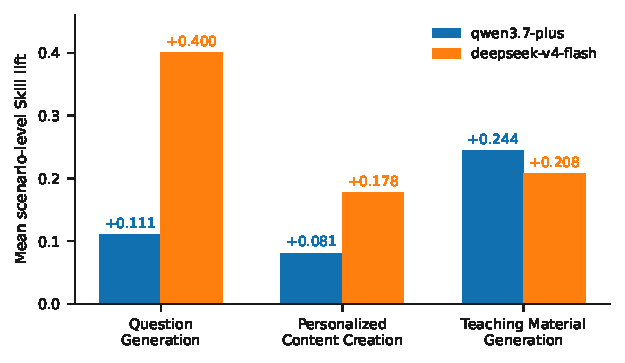
\includegraphics[width=0.82\textwidth]{figure_6.pdf}
\caption{Scenario-level Skill lift on the evaluated single-turn subset. All three scenarios show positive aggregate lift for both models, but the relative ordering differs.}
\label{fig:scenariolifts}
\end{figure}

\subsection{Task- and Skill-Level Failure Modes}

By negative transfer we mean a Skill whose observed With-Skill reward is lower than its matched No-Skill baseline. This usage follows the Agent-Skills literature \cite{skillsbench} and is distinct from the learning-science sense of prior learning interfering with new learning.

The strongest Qwen beneficiary is \skill{lesson-builder} (+0.733), followed by \skill{project-brief-designer} (+0.600) and \skill{socratic-questioning-sequence-generator} (+0.467). The only Qwen negative case is \skill{hinge-question-designer} ($-0.400$), whose No-Skill baseline already scores 1.000.

For DeepSeek, the strongest beneficiary is \skill{retrieval-practice-generator} (+0.867), followed by \skill{ruler-emotional-literacy-sequence} (+0.667) and \skill{adaptive-hint-sequence-designer} (+0.600). The only negative case is \skill{lesson-builder} ($-0.267$).

These results expose two recurring benchmark phenomena. First, a Skill may over-constrain or displace a strategy that already works well for a model. Second, Skill instructions that are helpful to one model may be too complex, too rigid, or poorly internalized by another. Distinguishing content quality from adherence requires trajectory-level analysis, which is not yet part of the released v1 score, and distinguishing these explanations from single-run noise requires the repeated-run validation in Section~6.1.

\section{Discussion}

\textbf{The largest observed gains occur on tasks that require structured educational procedures.}
Retrieval practice design, lesson planning, adaptive hinting, project briefing, and Socratic questioning are all tasks with explicit procedural structure. This pattern is consistent with the intended role of Skills as reusable procedures rather than factual context. The current experiment does not, however, directly separate procedural benefit from instruction-following or added context. That separation requires the instruction-level control and adherence diagnostics described in Section~6.1, so we state the pattern as consistent with, not evidence for, the mechanism.

\textbf{Skill evaluation should report more than an average.}
The observed cross-model reversals show why a single benchmark mean is insufficient. A useful Skill benchmark should report per-Skill lift, negative transfer, ceiling effects, and scenario variation. In future versions, we also plan to report explicit Skill adherence and interaction-quality diagnostics.

\textbf{Rubric design interacts with the measured lift.}
Because tasks and rubrics are aligned to the matched Skill, the measured lift is bounded below by the benefit of expressing the Skill's own procedure. This makes \bench's headline numbers interpretable as Skill-aligned utility, and it makes the interaction between rubric design and observed lift a first-class measurement target. Reporting the lift without the Skill execution family, and validating rubrics against independent human judgment, will tell us how much of the observed benefit is pedagogical rather than structural.

\textbf{Task-specific rubrics are essential in education.}
Unlike terminal tasks with deterministic test suites, educational artifacts often admit multiple valid outputs. A rubric must therefore encode pedagogical requirements, not only correctness. \bench~treats those rubrics as part of the benchmark specification rather than as post-hoc evaluation prompts.

\textbf{Public-only Skill sourcing improves ecological validity.}
Because the benchmark does not invent Skills to fill missing scenarios, coverage reflects the public Skill ecosystem rather than an idealized taxonomy. The trade-off is uneven coverage: Teaching Material Generation is overrepresented, while three EduBench-inspired scenarios remain uncovered.

\textbf{Cross-model Skill behavior is itself an evaluation target.}
Qwen and DeepSeek both benefit overall, yet the per-Skill patterns are not interchangeable. Because each model row was scored by a same-family judge, we treat the cross-model pattern as descriptive pending common-judge validation. If it survives that validation, future Skill benchmarks should treat the model--Skill pair, not the Skill alone, as the unit of practical deployment evaluation.

\subsection{Limitations and Required Validation Experiments}

We separate the limitations of the current release from the experiments required to move the claims beyond descriptive observation. The limitations are known and disclosed; the validation experiments are the specific actions that would close them.

\textbf{Known limitations of the v1 release.}

\begin{itemize}
  \item \textbf{Limited scale.} The current inventory contains 54 tasks and only three cases per Skill. The observed deltas are therefore sensitive to individual task instances.
  \item \textbf{Single-run reporting.} Each task-condition cell has one final clean result. We report point estimates and do not claim precision, significance, or confidence intervals for any headline value.
  \item \textbf{Judge dependence.} The current model rows use model-specific LLM judges. Paired lifts within a row are informative, but absolute scores across rows can be affected by judge calibration, and LLM-as-a-judge position, verbosity, and self-enhancement biases \cite{llmjudge} are directly relevant because With-Skill outputs are likely longer and more structured.
  \item \textbf{Skill-aligned task construction.} Tasks are deliberately written around the behavior each Skill claims to support, and the single-turn reward includes a Skill execution family. This measures Skill-aligned utility, not average value over arbitrary educational work, and it may reward structure that resembles the Skill.
  \item \textbf{Skill versus added instructions.} The No-Skill arm adds no instruction text, so the experiment does not separate the Skill as a reusable package from the effect of adding task-relevant instructions of comparable length.
  \item \textbf{Mechanism not directly measured.} The current score cannot separate content quality from adherence to the Skill procedure; the manuscript states this itself in Section~5.3.
  \item \textbf{Multi-turn evaluation is not yet reported.} Twelve multi-turn task specifications are released, but a dedicated stateful learner--agent protocol is still required before they can be scored comparably.
  \item \textbf{Incomplete scenario coverage.} Six of nine EduBench-inspired scenarios are represented. We intentionally avoid inventing new Skills solely to improve coverage.
  \item \textbf{Source drift and model aliases.} Public Skill repositories and API-served model aliases can change. Reproducible releases should pin upstream commits and model snapshots whenever possible.
\end{itemize}

\textbf{Required validation experiments.}
Each item below is a concrete, runnable specification. None of the observed numbers in this paper depend on these experiments; they are the work required to upgrade the claims from descriptive to causal and uncertainty-bounded.

\begin{itemize}
  \item \textbf{E1. Repeated runs and uncertainty bounds.} Run each of the 42 single-turn task-condition cells at least three times under controlled seeds. Report per-cell and per-Skill means with standard deviations and a bootstrap confidence interval over the three cases per Skill, and a paired test (for example a Wilcoxon signed-rank test over the 42 No-Skill versus With-Skill pairs per model) for the aggregate lift. Success criterion: the headline \ppgain{18.1} and \ppgain{24.3} lifts, the 10-of-14 and 9-of-14 classifications, and the one-negative-per-model pattern survive with quantified uncertainty.
  \item \textbf{E2. Common independent judge and human validation.} Score a shared stratified sample of both models' No-Skill and With-Skill outputs with a single third-party judge and with human raters. Report inter-judge agreement (for example Cohen's kappa or intraclass correlation) and a judge-bias analysis. Success criterion: cross-model lift patterns and reversals replicate under the common judge, or the judge-confound explanation is quantified and controlled.
  \item \textbf{E3. Matched-length instruction control.} Add two control arms over the same 42 tasks: matched-length generic instructions with no Skill, and a non-matched public Skill of comparable length. Compare the With-Skill lift against both. Success criterion: the With-Skill lift exceeds the instruction-only baseline by a margin beyond the E1 intervals; otherwise the claim narrows to the effect of adding Skill-sourced instructions.
  \item \textbf{E4. Rubric de-coupling.} Re-score outputs with the Skill execution family removed or blinded, and validate rubrics against independent human judgments of pedagogical quality on a sample (for example three tasks per Skill). Optionally add tasks in the same scenarios that are not aligned to any Skill. Success criterion: a material lift persists without the Skill execution family, and human-judged pedagogical quality moves with the With-Skill advantage.
  \item \textbf{E5. Trajectory-level adherence analysis.} Score agent traces for adherence to the Skill procedure separately from output quality, and report the adherence by outcome interaction. This turns the Section~5.3 caveat into a measurement.
  \item \textbf{E6. Timeout sensitivity.} Re-run the four affected DeepSeek With-Skill cells and their No-Skill counterparts under a uniform 600-second timeout, and report both conditions.
\end{itemize}

Beyond these, future versions should expand the task inventory, run the multi-turn subset, and test retrieval from larger noisy Skill libraries rather than assuming a perfectly matched Skill.

\section{Related Work}

\textbf{Education-facing benchmarks.}
EduBench defines nine educational scenarios and multidimensional criteria for education-oriented LLM evaluation \cite{edubench}. LearnLM studies pedagogical instruction following in education-focused model development \cite{learnlm}, while Tutor CoPilot shows that structured AI guidance can change tutoring behavior in real instructional settings \cite{tutorcopilot}. \bench~differs by evaluating reusable public Agent Skills as the intervention.

\textbf{Agent Skills and augmentation evaluation.}
SkillsBench establishes broad paired evaluation for curated Skills and reports substantial but heterogeneous gains across model--harness configurations \cite{skillsbench}. \bench~adopts the paired-condition principle but specializes task and rubric construction to educational procedures and open-ended outputs, and it reports the Skill-aligned nature of that construction as an explicit design feature.

\textbf{Rubric-based LLM evaluation.}
LLM-as-a-judge methods provide a scalable approach for evaluating open-ended model outputs but can exhibit position, verbosity, and self-enhancement biases \cite{llmjudge}. These limitations motivate our explicit expected-behavior rubrics and the planned addition of a common judge and independent human validation (Section~6.1, E2).

\section{Conclusion}

We introduced \bench, a benchmark for evaluating reusable public Agent Skills on educational tasks. The v1 release contains 18 Skills and 54 tasks, with explicit task-specific rubrics and six EduBench-inspired scenarios. On the 42-task single-turn subset, matched Skills are associated with an observed increase in mean rubric reward from 0.767 to 0.948 for \texttt{qwen3.7-plus} and from 0.314 to 0.557 for \texttt{deepseek-v4-flash}, reported as single-run point estimates. The gains are substantial but model-specific, with one negative-transfer Skill in each configuration and several ceiling-limited cases.

The main lesson is conditional: educational Skills can provide meaningful support in the tested conditions, but their value cannot be inferred from the Skill text alone. It must be measured against a specific model, task, rubric, and harness, and it must be bounded by repeated runs and a common judge before the cross-model conclusions can be read causally. By releasing Skills, task specifications, rubrics, evaluation scripts, and results, \bench~provides a foundation for broader evaluation of Skill-augmented educational agents. The multi-turn subset is released as specifications and is not yet evaluated.

\appendix

\section{Complete Per-Skill Results}

\begin{table}[H]
\centering
\scriptsize
\caption{Complete single-turn per-Skill results. Values are mean normalized rubric rewards over three cases (0 to 1 scale), single-run point estimates, read directly from the release results files. Qwen columns are from \texttt{results/single\_turn\_skill\_summary.csv}; DeepSeek columns are from the \texttt{formal-deepseek-v4-flash} runs merged with the four 600-s rerun cells disclosed in Section~4.2 (lesson-builder, self-efficacy-builder-sequence, socratic-questioning-sequence-generator, emergent-project-design-scaffold, With-Skill arms only). $\Delta$ = With $-$ No. These per-Skill cells reproduce the Table~3 aggregates exactly (Qwen macro mean of $\Delta$ $+0.181$; DeepSeek $+0.243$).}
\label{tab:fullskill}
\begin{tabularx}{0.99\textwidth}{>{\ttfamily\raggedright\arraybackslash}Xrrrrrr}
\toprule
& \multicolumn{3}{c}{Qwen3.7-Plus} & \multicolumn{3}{c}{DeepSeek-V4-Flash}\\
\cmidrule(lr){2-4}\cmidrule(lr){5-7}
Skill & No & With & $\Delta$ & No & With & $\Delta$\\
\midrule
adaptive-hint-sequence-designer & 0.800 & 0.867 & +0.067 & 0.000 & 0.600 & +0.600 \\
backwards-design-unit-planner & 1.000 & 1.000 & 0.000 & 1.000 & 1.000 & 0.000 \\
differentiation-adapter & 1.000 & 1.000 & 0.000 & 0.933 & 1.000 & +0.067 \\
emergent-project-design-scaffold & 0.650 & 1.000 & +0.350 & 0.000 & 0.000 & 0.000 \\
hinge-question-designer & 1.000 & 0.600 & $-0.400$ & 0.333 & 0.333 & 0.000 \\
lesson-builder & 0.200 & 0.933 & +0.733 & 0.267 & 0.000 & $-0.267$ \\
motivation-diagnostic-task-redesign & 0.867 & 1.000 & +0.133 & 0.533 & 0.667 & +0.133 \\
project-brief-designer & 0.400 & 1.000 & +0.600 & 0.000 & 0.333 & +0.333 \\
retrieval-practice-generator & 0.733 & 1.000 & +0.267 & 0.133 & 1.000 & +0.867 \\
ruler-emotional-literacy-sequence & 0.733 & 0.867 & +0.133 & 0.267 & 0.933 & +0.667 \\
self-efficacy-builder-sequence & 0.890 & 1.000 & +0.110 & 0.000 & 0.333 & +0.333 \\
self-explanation-prompt-designer & 1.000 & 1.000 & 0.000 & 0.600 & 0.600 & 0.000 \\
socratic-questioning-sequence-generator & 0.533 & 1.000 & +0.467 & 0.000 & 0.333 & +0.333 \\
spaced-practice-scheduler & 0.933 & 1.000 & +0.067 & 0.333 & 0.667 & +0.333 \\
\midrule
\textbf{Mean} & \textbf{0.767} & \textbf{0.948} & \textbf{+0.181} & \textbf{0.314} & \textbf{0.557} & \textbf{+0.243} \\
\bottomrule
\end{tabularx}
\par\vspace{4pt}
{\footnotesize\textbf{Data provenance.} All seven cells quoted in Section~5.3 and Findings~2--3 (Qwen lesson-builder $+0.733$, hinge-question $-0.400$, project-brief $+0.600$, socratic $+0.467$, retrieval $+0.267$; DeepSeek retrieval $+0.867$, ruler-emotional $+0.667$, adaptive-hint $+0.600$, lesson-builder $-0.267$) match the values above to $\pm 0.001$. The per-Skill macro means equal the Table~3 aggregates for both models, confirming the per-Skill and aggregate tables were generated from the same result set.}
\end{table}

\section{Skill Inventory and Scenario Mapping}

\begin{table}[H]
\centering
\small
\caption{The 18 retained Skills and their EduBench-inspired scenarios.}
\begin{tabularx}{0.98\textwidth}{>{\ttfamily\raggedright\arraybackslash}Xll}
\toprule
Skill & Scenario & Interaction \\
\midrule
retrieve-first-gate & Q\&A & multi-turn \\
stuck-and-error-diagnosis-coach & Error Correction & multi-turn \\
progressive-hint-ladder & Personalized Learning Support & multi-turn \\
confidence-calibration-check & Personalized Learning Support & multi-turn \\
hinge-question-designer & Question Generation & single-turn \\
retrieval-practice-generator & Question Generation & single-turn \\
socratic-questioning-sequence-generator & Question Generation & single-turn \\
differentiation-adapter & Personalized Content Creation & single-turn \\
motivation-diagnostic-task-redesign & Personalized Content Creation & single-turn \\
self-efficacy-builder-sequence & Personalized Content Creation & single-turn \\
backwards-design-unit-planner & Teaching Material Generation & single-turn \\
lesson-builder & Teaching Material Generation & single-turn \\
adaptive-hint-sequence-designer & Teaching Material Generation & single-turn \\
self-explanation-prompt-designer & Teaching Material Generation & single-turn \\
emergent-project-design-scaffold & Teaching Material Generation & single-turn \\
project-brief-designer & Teaching Material Generation & single-turn \\
spaced-practice-scheduler & Teaching Material Generation & single-turn \\
ruler-emotional-literacy-sequence & Teaching Material Generation & single-turn \\
\bottomrule
\end{tabularx}
\end{table}

\section{Released Task Example}

The released task \texttt{hinge-question-designer\_\_01} is a Grade 8 biology Question Generation case. The teacher has just covered photosynthesis and asks for a two-minute multiple-choice checkpoint before moving to cellular respiration. The requested output must include the question, four options, the correct answer, a misconception diagnosis for each distractor, a decision guide for teaching next steps, and a design rationale. Its five rubric criteria evaluate (1) stem and option quality, (2) diagnostic distractors, (3) diagnostic-key accuracy, (4) actionability of the decision guide, and (5) design rationale. This illustrates how \bench~evaluates both the educational artifact and the procedure used to construct it. It also illustrates the Skill-aligned construction disclosed in Section~3.5: criteria (2) through (4) reward exactly the structure a hinge-question Skill is designed to produce.

\section{Reproducibility Notes}

The main repository is \url{https://github.com/Airlivy/EduSkillBench}. It releases task specifications, Skill mappings, Skill packages, generation scripts, evaluation scripts, aggregate results, and licensing notices. Runtime job directories, API credentials, and local caches are excluded.

The Qwen experiment uses the API identifier \texttt{qwen3.7-plus}; the underlying provider snapshot is not independently pinned. DeepSeek is evaluated as \texttt{deepseek-v4-flash}. Both use OpenCode and Docker through BenchFlow. The release includes a compatibility patch for the BenchFlow version used in the original environment when routing a custom OpenAI-compatible endpoint and preserving a non-default judge identifier.

For the revised release we commit to the following additions, which close the reproducibility gaps identified in review:
\begin{itemize}
  \item A version manifest pinning the upstream Skill repository commits, the provider snapshots (or explicit model-version identifiers), and the exact \texttt{qwen3.7-plus} and \texttt{deepseek-v4-flash} API identifiers used.
  \item The full judge specification, including the judge prompt, temperature, sampling parameters, the judge's input fields, and whether the judge sees the rubric and the matched Skill.
  \item A machine-readable per-Skill results table (provided; see Appendix~A, Table~\ref{tab:fullskill}, which reproduces the Table~3 aggregates for both models) and per-task raw rewards for every evaluated cell.
  \item The evaluation timestamps and the exact DeepSeek timeout handling, including which cells were rerun and under which limit.
\end{itemize}

\begin{thebibliography}{99}

\bibitem{skillsbench}
Xiangyi Li, Yimin Liu, Wenbo Chen, et al.
\newblock SkillsBench: Benchmarking How Well Agent Skills Work Across Diverse Tasks.
\newblock \emph{arXiv:2602.12670v4}, 2026.

\bibitem{edubench}
Bin Xu, Yu Bai, Huashan Sun, Yiguan Lin, Siming Liu, Xinyue Liang, Yaolin Li, Zhuangzhi Dong, Jingren Zhang, Yufan Deng, Xinyu Zou, Yang Gao, and Heyan Huang.
\newblock EduBench: A Comprehensive Benchmarking Dataset for Evaluating Large Language Models in Diverse Educational Scenarios.
\newblock \emph{arXiv:2505.16160}, 2025.

\bibitem{llmjudge}
Lianmin Zheng, Wei-Lin Chiang, Ying Sheng, Siyuan Zhuang, Zhanghao Wu, Yonghao Zhuang, Zi Lin, Zhuohan Li, Dacheng Li, Eric P. Xing, Hao Zhang, Joseph E. Gonzalez, and Ion Stoica.
\newblock Judging LLM-as-a-Judge with MT-Bench and Chatbot Arena.
\newblock \emph{NeurIPS}, 2023.

\bibitem{hake}
Richard R. Hake.
\newblock Interactive-engagement versus traditional methods: A six-thousand-student survey of mechanics test data for introductory physics courses.
\newblock \emph{American Journal of Physics}, 66(1):64--74, 1998.

\bibitem{learnlm}
LearnLM Team, Abhinit Modi, Aditya Srikanth Veerubhotla, et al.
\newblock LearnLM: Improving Gemini for Learning.
\newblock \emph{arXiv:2412.16429}, 2024.

\bibitem{tutorcopilot}
Rose E. Wang, Ana T. Ribeiro, Carly D. Robinson, Susanna Loeb, and Dora Demszky.
\newblock Tutor CoPilot: A Human-AI Approach for Scaling Real-Time Expertise.
\newblock \emph{arXiv:2410.03017}, 2024.

\bibitem{educationagentskills}
Gareth Manning.
\newblock Education Agent Skills Library.
\newblock \url{https://github.com/GarethManning/education-agent-skills}, accessed 2026.

\bibitem{teachingskills}
YujxZJCN.
\newblock Teaching Skills.
\newblock \url{https://github.com/YujxZJCN/teaching-skills}, accessed 2026.

\bibitem{benchflow}
BenchFlow Team.
\newblock BenchFlow: an environment framework for evaluating AI agents.
\newblock \url{https://github.com/benchflow-ai/benchflow}, 2026.

\end{thebibliography}

\end{document}
